\chapter{Assemblaggio della scheda}

L’assemblaggio della scheda è stato svolto in laboratorio sotto la supervisione
del Professore presso il laboratorio di elettronica del FabLab. 
In seguito all’arrivo delle PCB e dei componenti principali, abbiamo 
deposto la pasta saldante sulla scheda con l’aiuto dello stencil serigrafico
per procedere con la saldatura dei componenti con metodo \emph{thermal reflow}.\\
Al fine di tenere la scheda in posizione fissa, questa è stata inserita 
tra altre 4 schede fissate sul banco. Dopo aver passato la pasta saldante, 
abbiamo successivamente posizionato con particolare attenzione i componenti 
sulla scheda, controllando accuratamente il layout progettato in precedenza
ed aiutandoci con la BOM interattiva (che associa refdes e valore del componente
alla propria posizione sulla PCB).\\
Alcuni dei componenti realmente utilizzati
presentavano un modello diverso da quello previsto in fase di progettazione ma,
essendo una scheda di prototipazione e non una scheda di produzione, sono
risultati ugualmente adatti, senza alterare il funzionamento della scheda.
Infine, abbiamo fissato i componenti utilizzando una stazione di saldatura 
con piastra elettrica riscaldante, permettendo lo scioglimento delle sfere 
di stagno (contenute all’interno della pasta) e la conseguente saldatura 
dei dispositivi SMD.\\
Finito l’assemblaggio, ci siamo accorti che per una 
particolare scheda i pin del microcontrollore non sembravano essere fissati a
dovere ed infatti testando la sua alimentazione abbiamo potuto constatare il
surriscaldamento eccessivo del componente. Perciò per rimediare all’errore il
microcontrollore è stato dissaldato, ma nel farlo, le tre piste che collegavano
i rispettivi pin si sono alzate, non consentendo così l’utilizzo della scheda.\\
Un altro errore è sorto durante la fase di testing, infatti, misurando il 
segnale di comando in input ai motori, ci siamo accorti che al transistor a 
canale N montato sulla scheda era stata assegnata la piedinatura scorretta. 
Pertanto, abbiamo dovuto dissaldare i transistor atti al pilotaggio dei motori
per poi saldarli nuovamente nel verso corretto.


\begin{center}
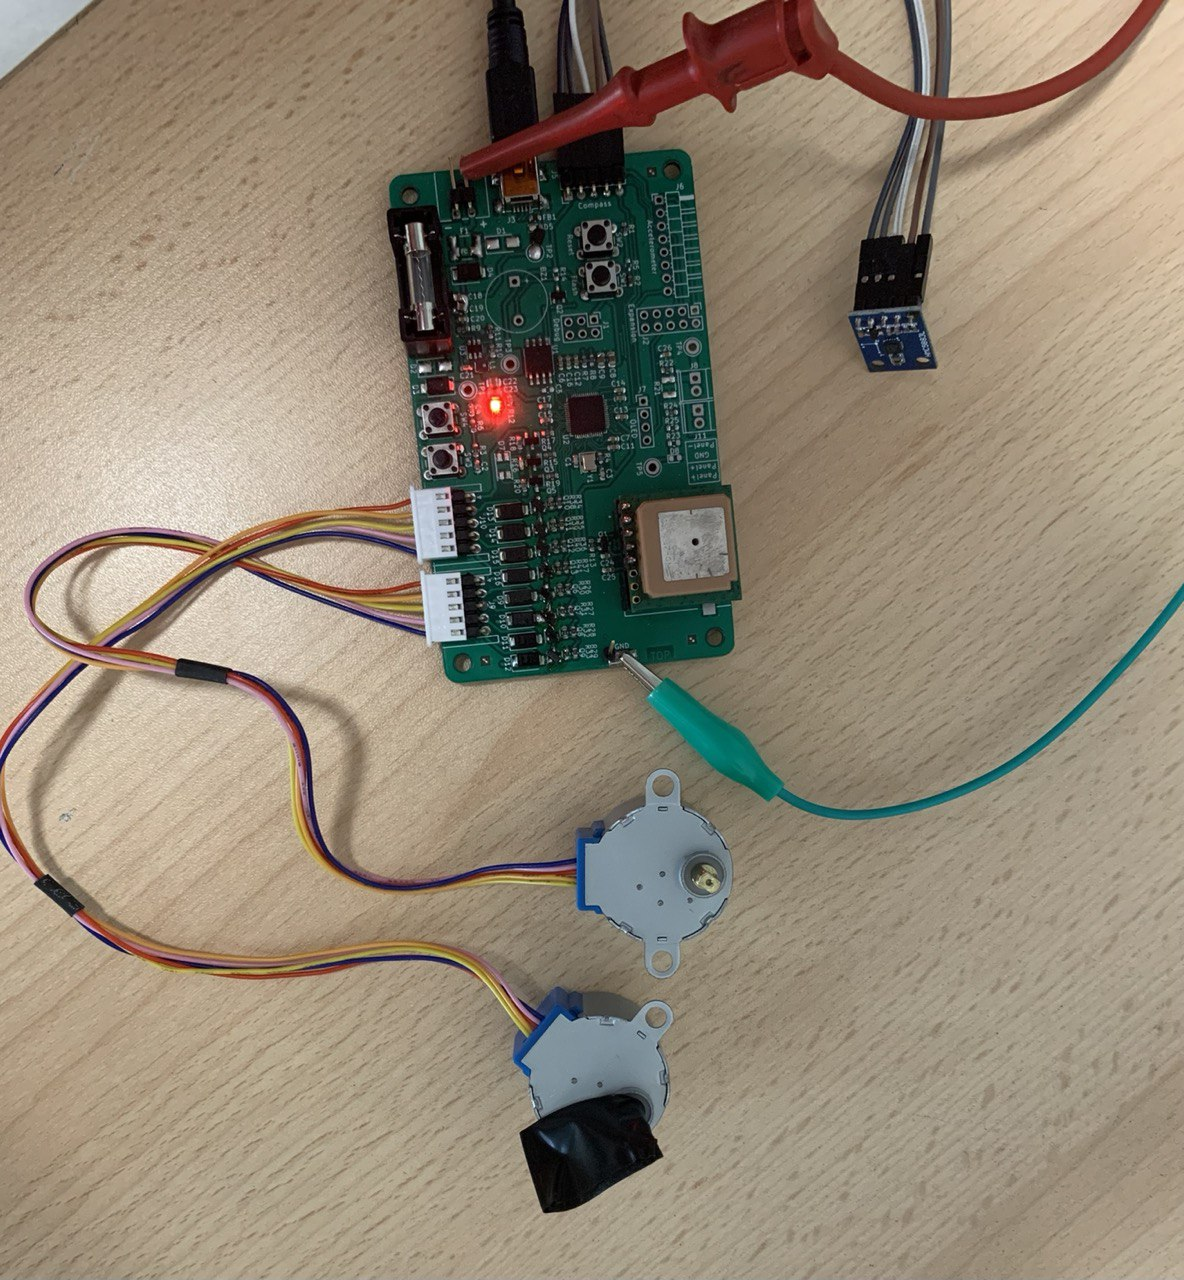
\includegraphics[scale=0.4]{figures/image101.png}
\captionsetup{type=figure}
\captionof{figure}{Scheda SALMO completa di componenti essenziali}
\end{center}